\documentclass[a4paper,12pt]{article}

\usepackage[T2A]{fontenc}			
\usepackage[utf8]{inputenc}			
\usepackage[english,russian]{babel}	

\usepackage[
bookmarks=true, colorlinks=true, unicode=true,
urlcolor=black,linkcolor=black, anchorcolor=black,
citecolor=black, menucolor=black, filecolor=black,
]{hyperref}

\usepackage{color}
\usepackage{caption}
\DeclareCaptionFont{white}{\color{black}}
\DeclareCaptionFormat{listing}{\colorbox{white}{\parbox{\textwidth}{#1#2#3}}}
\captionsetup[lstlisting]{format=listing,labelfont=white,textfont=white}

\usepackage{amsmath,amsfonts,amssymb,amsthm,mathtools} 
\usepackage{wasysym}

\usepackage{graphicx}
%\usepackage[cache=false]{minted}
\usepackage{cmap}
\usepackage{indentfirst}

\usepackage{listings} 
\usepackage{fancyvrb}

\usepackage{geometry}
\geometry{left=2cm}
\geometry{right=1.5cm}
\geometry{top=1cm}
\geometry{bottom=2cm}

\setlength{\parindent}{5ex}
\setlength{\parskip}{0.5em}

\usepackage{pgfplots}

\usepackage{longtable}

\begin{document}
	\lstset{ %
		language=C,                 % выбор языка для подсветки (здесь это С)
		basicstyle=\small\sffamily, % размер и начертание шрифта для подсветки кода
		numbers=left,               % где поставить нумерацию строк (слева\справа)
		numberstyle=\tiny,           % размер шрифта для номеров строк
		stepnumber=1,                   % размер шага между двумя номерами строк
		numbersep=5pt,                % как далеко отстоят номера строк от подсвечиваемого кода
		backgroundcolor=\color{white}, % цвет фона подсветки - используем \usepackage{color}
		showspaces=false,            % показывать или нет пробелы специальными отступами
		showstringspaces=false,      % показывать или нет пробелы в строках
		showtabs=false,             % показывать или нет табуляцию в строках
		frame=single,              % рисовать рамку вокруг кода
		tabsize=2,                 % размер табуляции по умолчанию равен 2 пробелам
		captionpos=t,              % позиция заголовка вверху [t] или внизу [b] 
		breaklines=true,           % автоматически переносить строки (да\нет)
		breakatwhitespace=false, % переносить строки только если есть пробел
		escapeinside={\%*}{*)}   % если нужно добавить комментарии в коде
	}
	
	% Титульный лист
	\begin{figure}[h!]
		\begin{center}
			{\includegraphics[scale = 0.4]{titul.jpg}}
			\label{titul}
		\end{center}
	\end{figure}
	
	\vspace*{15mm} 
	
	\huge
	\begin{center}
		Дисциплина: <<Моделирование>>
	\end{center}
	
	\begin{center}
		Лабораторная работа №6
	\end{center}

	
	\huge
	\begin{center}
		Тема работы:\\
		<<Моделирование работы кинотеатра>>
	\end{center}
	\vspace*{25mm} 
	
	\large
	\begin{flushright}
		Студент: Левушкин И. К. \\
		Группа: ИУ7-72Б \\
		Преподаватель: Рудаков И. В. \\
	\end{flushright}
	
	\vspace*{25mm}
	\begin{center}
		Москва, 2020 г.  
	\end{center}
	\thispagestyle{empty}
	
	
	\newpage
	
	\section*{Задание}
	
	Смоделировать работу кинотеатра. Посетители приходят через 2 входа через интервал времени $8 \pm 2$ минуты, затем осуществляется досмотр в 3 потока за $10 \pm 3$ и $11 \pm 1$ и $12 \pm 2$, соответственно. После чего посетители отправляются на одну из четырех касс с временем обслуживания $11 \pm 3$, $14 \pm 1$,  $16 \pm 3$ и $27 \pm 2$, соответственно. Далее, они отправляются в кинозал, где принимают билеты 2 проверяющих со скоростью обслуживания $4 \pm 1$ и $6 \pm 2$, соответственно. Также, при покупке билетов и входе в кинозал существует вероятность 10\%, что посетителю откажут (по причине неадекватного поведения, ограничений по возрасту или проносу еды).
	Во всех случаях посетители стараются занять очередь с минимальным числом людей.
	
	Определить максимальное время ожидания в каждой из очередей и их максимальные длины.
	Количество мест в кинозале равно 150.
	
	\newpage
	
	\section*{Формализация}
	
	\subsection*{Концептуальная модель}
	
	Ниже приведена концептуальная модель в терминах СМО.
	
	\begin{figure}[h!]
		\begin{center}
			{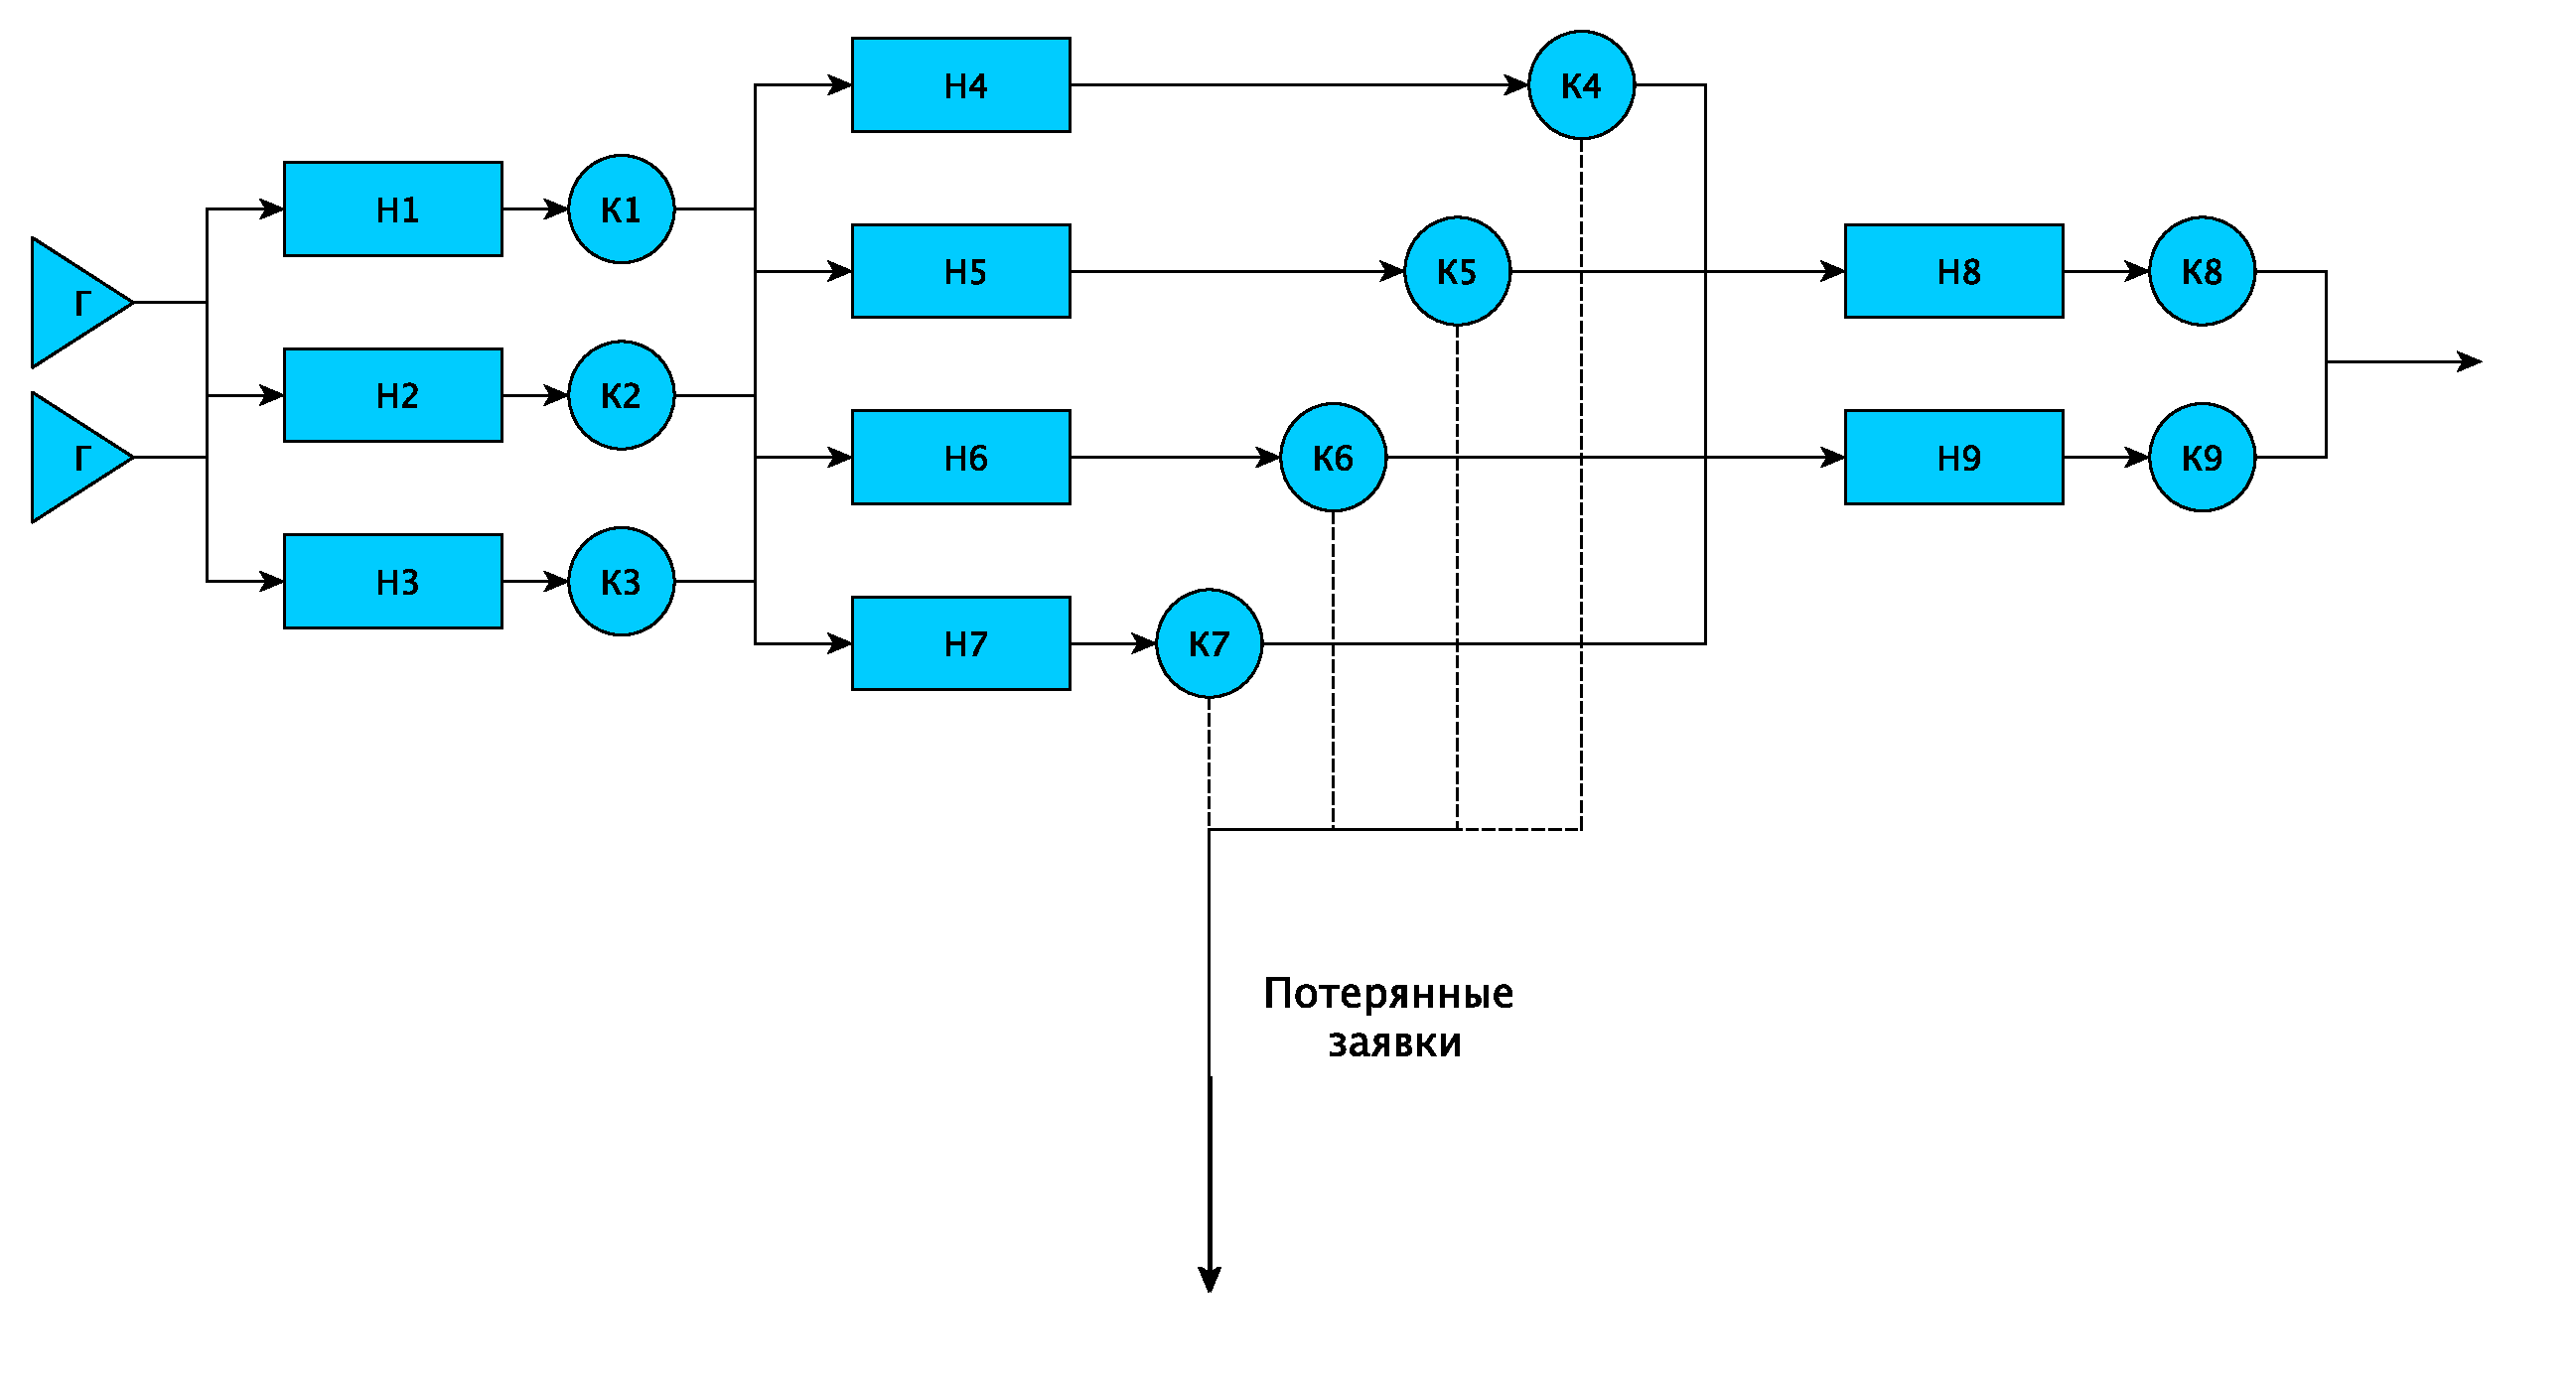
\includegraphics[scale = 0.4]{model.pdf}}
			\label{ris:model}
		\end{center}
		\caption{Концептуальная модель в терминах СМО.}
	\end{figure}
	
	\subsection*{Эндогенные и экзогенные переменные имитационной модели}
	
	{\bf Эндогенные переменные} - время проверки посетителя $i$-ым охранником,
	время оформления билета $j$-ым сотрудником, время проверки билета посетителя $k$-ым билетером.
	
	{\bf Экзогенные переменные} - число посетителей, пришедших в кинозал.
	
	\newpage
	
	\section*{Результаты работы}
	
	В данной работе для моделирования кинотеатра выбран событийный принцип.
	
	Ниже приведены результаты работы программы.
	
	\begin{figure}[h!]
		\begin{minipage}[b]{0.48\textwidth}
			\includegraphics[width=\textwidth]{1.png}
		\end{minipage}
		\begin{minipage}[b]{0.48\textwidth}
			\includegraphics[width=\textwidth]{2.png}
		\end{minipage}
		\center{СМО кинотеатра}
		\label{ris:smo1}
	\end{figure}

	\begin{figure}[h!]
		\begin{center}
			{\includegraphics[scale = 0.4]{3.png}}
			\label{ris:smo2}
		\end{center}
		\caption{СМО кинотеатра.}
	\end{figure}

	
	
	\section*{Вывод}
	
	Проведено имитационное моделирование кинотеатра с использованием событийного метода.
	
	В результате проделанной работы была проведена формализация задачи, на основе чего была разработана программа, реализующая поставленную задачу.
	
	Программа позволяла определить максимальное время ожидания в каждой из очередей и их максимальные длиныи.
	
\end{document}